% Results for Paper A. Primary corpus: GNPS + MassBank + MoNA (open, 66 instrument
% types). Secondary: the single-library corpus, which supplies a replication under
% very different acquisition diversity plus the bin-width sweep.
\section*{Results}

\hd{The five arms}
The design is a ladder in which each arm differs from the one below it in exactly
one respect (Table~\ref{tab:table1_arms_open}). M0 is the conventional baseline: a
$0.5$~Da binned intensity vector read by a two-layer perceptron, with the
acquisition covariates concatenated to that vector so the baseline sees the same
conditioning information as every other arm (Sect.~\ref{sec:fair}). M1D keeps that binned mass axis but
presents the spectrum as a set of peak tokens rather than one dense vector: each
peak is snapped to its bin centre, colliding peaks are merged, and the tokens pass
through a position-wise network with no attention, pooled by a masked mean. M1R
adds self-attention to those same tokens. M1 hands the same attentive encoder the
peaks at full precision. M2 adds hierarchical pooling over a molecule's spectra. M1R and M1 are identical in every configuration field but
the width of the mass grid, and carry identical parameter counts; M1D differs from
M1R only in carrying no attention, with its feed-forward widened so that it is not
also the smaller arm ($714{,}528$ parameters against $712{,}336$). Each arm was
trained three times, under seeds $\{2026, 7, 13\}$.

M1R is the rung that makes the experiment mean anything. Without it, the contrast
between a binned baseline and a peak-set model changes the mass axis and the encoder
together, and a difference between them cannot be assigned to either. M1D then
splits the encoder itself, separating the change of interface --- peaks presented
individually rather than summed into a dense vector --- from the attention built on
top of it.

\begin{table}[htbp]
\centering
\caption{The four arms on the open corpus, each differing from the one above it in a single respect. Macro AUPRC on 10,058 held-out molecules, mean over three seeds. Chance is 0.0085 over 433 scored targets.}
\label{tab:table1_arms_open}
\begin{tabular}{l r r r r r r}
\toprule
arm & mass axis & encoder & pooling & parameters & macro AUPRC & SD over seeds \\
\midrule
M0 & 0.5 Da bins & MLP & mean & 1,164,560 & 0.1130 & 0.0012 \\
M1R & 0.5 Da bins & Transformer & mean & 712,336 & 0.1567 & 0.0025 \\
M1 & full precision & Transformer & mean & 712,336 & 0.1709 & 0.0022 \\
M2 & full precision & Transformer & hierarchical & 829,584 & 0.1888 & 0.0015 \\
\bottomrule
\end{tabular}
\end{table}


\hd{Half of the apparent advantage is the baseline's missing metadata}
\label{sec:fair}
Our first version of this experiment reproduced the standard baseline faithfully,
and that turned out to include a handicap we had not intended. The binned encoder
took the acquisition covariates as an argument and never used them, so M0 alone
could not see the collision energy, adduct, polarity or instrument, while every
peak-set arm conditioned each of its blocks on them. Collision energy largely
determines which bonds break, so a model blind to it must marginalise over every
energy in the corpus.

Concatenating the same covariate embedding to the binned vector raises M0 from
$0.1130$ to $0.1418$, an improvement of $+0.0288$ --- larger than any of the three
effects this paper set out to measure. The gap a two-arm comparison would report
falls with it, from $+0.0579$ to $+0.0291$. Half of what looked like the advantage
of reading peaks at full precision was the baseline not being told how the spectrum
was acquired.

We report this because it is the paper's own thesis turned on the paper. Every
number below is measured against the conditioned baseline.

\hd{Against a fair baseline, the encoder and the mass axis are worth the same}
Replacing the binned vector with a full-precision peak set raises macro AUPRC from
$0.1418$ to $0.1709$ against a chance level of $0.0085$, a paired per-target gain of
$+0.0291$ ($95\%$ CI $+0.0208$ to $+0.0371$) improving $72.5\%$ of targets. The
control splits it (Fig.~\ref{fig:decomposition},
Table~\ref{tab:table2_effects_open}). Changing the encoder alone, with the mass axis
binned on both sides, is worth $+0.0149$ ($+0.0080$ to $+0.0221$; $66.7\%$ of
targets). Changing the mass axis alone, with the same encoder on both sides, is
worth $+0.0142$ ($+0.0097$ to $+0.0187$; $64.9\%$ of targets). The two sum to the
joint effect exactly, as they must, since each target's contribution enters both
sides linearly.

The two halves are therefore indistinguishable: $51\%$ encoder and $49\%$ mass axis.
Against the unconditioned baseline the same decomposition read $76\%$ and $24\%$.
Both components remain real, each interval excluding zero and each improving a clear
majority of targets, but the claim that one dominates the other does not survive a
baseline that has been told the collision energy.

\hd{Within the encoder, attention contributes nothing}
The encoder effect itself divides further. Presenting the spectrum as peak tokens
rather than one dense vector, with no attention anywhere in the network, is worth
$+0.0172$ ($+0.0102$ to $+0.0242$; $58.0\%$ of targets), and it holds in all three
seeds. Adding self-attention to those same tokens is worth $-0.0023$ ($-0.0066$ to
$+0.0020$), an interval straddling zero, improving $54.3\%$ of targets --- barely
more than half --- and positive in only one seed of three. The two sum to the
encoder effect exactly.

The interface accounts for $115\%$ of the encoder effect and attention for $-15\%$.
We do not read the negative sign as evidence that attention hurts; we read the
interval as evidence that it does nothing measurable here. What matters is that a
position-wise perceptron over peak tokens captures the entire advantage that a
four-block Transformer over the same tokens captures, at a parameter count slightly
in its favour.

This resolves a question the design left open in its first form. The contrast
between M0 and M1R changed both the interface and the network family, so part of
what we called ``the encoder'' might have been either. It is the interface.

\begin{table}[htbp]
\centering
\caption{Paired per-target differences on the open corpus, bootstrapped over targets after averaging each target's average precision across the three seeds. The interface and attention rows decompose the encoder row; the attention interval includes zero. The final column is the standard deviation of the effect across seeds.}
\label{tab:table2_effects_open}
\begin{tabular}{l r r r r r}
\toprule
contrast & isolates & $\Delta$ AUPRC & 95\% CI & targets improved & SD over seeds \\
\midrule
M1D $-$ M0 & interface & +0.0172 & [+0.0102, +0.0242] & 58.0\% & 0.0016 \\
M1R $-$ M1D & attention & -0.0023 & [-0.0066, +0.0020] & 54.3\% & 0.0023 \\
M1R $-$ M0 & encoder & +0.0149 & [+0.0080, +0.0221] & 66.7\% & 0.0013 \\
M1 $-$ M1R & mass axis & +0.0142 & [+0.0097, +0.0187] & 64.9\% & 0.0004 \\
M2 $-$ M1 & aggregation & +0.0179 & [+0.0136, +0.0223] & 63.7\% & 0.0009 \\
M1 $-$ M0 & encoder and mass axis & +0.0291 & [+0.0208, +0.0371] & 72.5\% & -- \\
M2 $-$ M0 & all three & +0.0470 & [+0.0377, +0.0566] & 73.9\% & -- \\
\bottomrule
\end{tabular}
\end{table}


\begin{figure}[htbp]
\centering
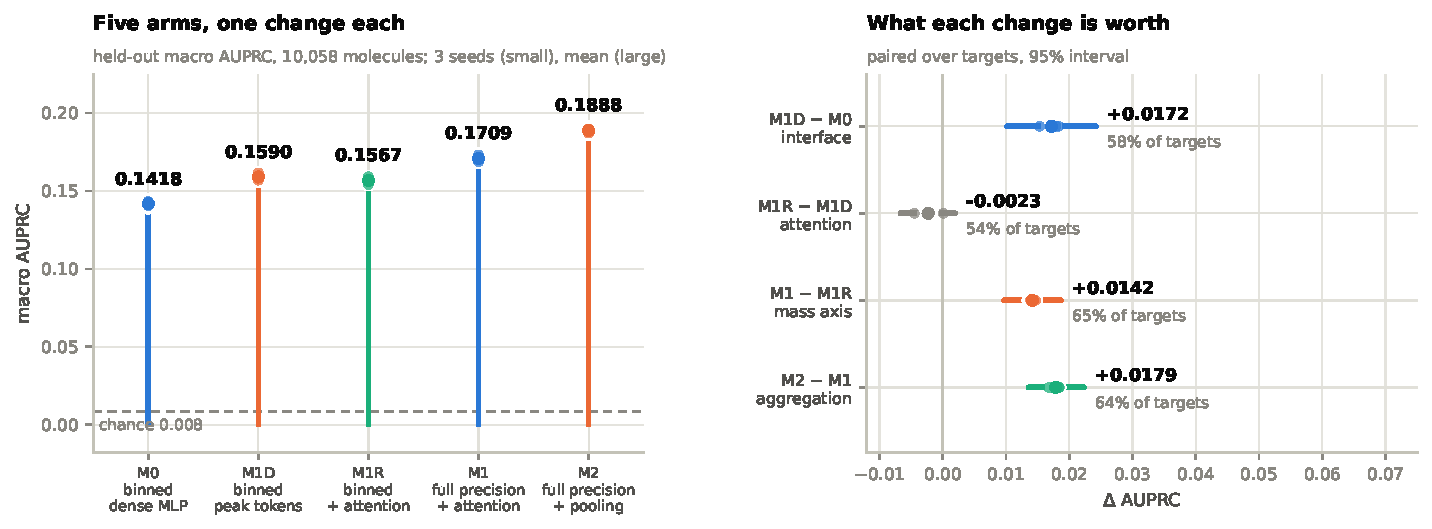
\includegraphics[width=\linewidth]{figures/fig1_decomposition_open.pdf}
\caption{Decomposing the gain on the open corpus. \textbf{Left}: held-out macro
AUPRC for the five arms; small dots are individual seeds, large dots their mean.
\textbf{Right}: what each single change is worth, paired over targets with $95\%$
bootstrap intervals; small dots are the per-seed effect sizes.}
\label{fig:decomposition}
\end{figure}

\hd{What the ordering supports, and what it no longer does}
Aggregation is now the largest of the three effects, exceeding the encoder in all
three seeds ($+0.0009$, $+0.0030$, $+0.0049$) and the mass axis in all three
($+0.0028$, $+0.0045$, $+0.0037$). It exceeds the encoder in all three seeds on the
single-library corpus as well. That ranking we regard as established.

The encoder and the mass axis cannot be separated. Their difference is $+0.0019$,
$+0.0015$ and $-0.0012$ across seeds: positive twice, negative once, and an order of
magnitude smaller than either effect. It reverses on the single-library corpus too,
in the opposite direction ($-0.0016$, $+0.0006$, $-0.0090$), so the failure to order
them is not a property of one corpus. Against the unconditioned baseline the encoder
led by $+0.0296$ and that ordering held in every seed. Conditioning the baseline
erased the lead.

The mass-axis effect remains the most precisely measured quantity in the study, with
a seed standard deviation of $0.0004$ against $0.0013$ for the encoder and $0.0009$
for aggregation. That the smallest effects here are also the most reproducible is
worth stating plainly: they are small effects measured precisely, not noise.


\hd{The same decomposition on a very different corpus}
The finding is a claim about how the field should construct comparisons, not about
one dataset. We therefore repeated the entire ladder on a second corpus with almost
nothing in common with the first. That corpus is a single in-house library, $99\%$
of whose spectra come from one instrument (timsTOF), against the open corpus's $66$
instrument types drawn from three public libraries
(Fig.~\ref{fig:corpora}, Table~\ref{tab:table3_two_corpora}).

Every effect is smaller on the open corpus, and by a similar factor: the encoder
falls from $+0.0234$ to $+0.0149$, the mass axis from $+0.0268$ to $+0.0142$, and
aggregation from $+0.0322$ to $+0.0179$. Both ladders were fitted against the
conditioned baseline, so all three contrasts are comparable.

What replicates is the finding, not merely its direction. On the single-library
corpus the encoder is worth $+0.0234$ and the mass axis $+0.0268$; their difference
is $-0.0016$, $+0.0006$ and $-0.0090$ across seeds, reversing sign exactly as it
does on the open corpus. The encoder's share of the gain a two-arm comparison would
report is $46.7\%$ here against $51.3\%$ there. Two corpora with almost nothing in
common --- one library against three, two instrument types against $66$, $16$
adducts against $112$ --- return the same answer: the encoder and the mass axis are
worth about the same, and neither can be ordered against the other. Aggregation
exceeds the encoder in all three seeds on both.

The correction itself replicates too, and in a way that supports the reading we give
it. Conditioning M0 on the acquisition covariates was worth $+0.0288$ on the open
corpus and $+0.0142$ on the single-library one. If those covariates matter because
they tell the model how the spectrum was produced, their value should scale with how
much the production varied, and the open corpus carries $66$ instrument types and
$112$ adducts against two and $16$. We offer this as a consistency check rather than
a result.

\begin{figure}[htbp]
\centering
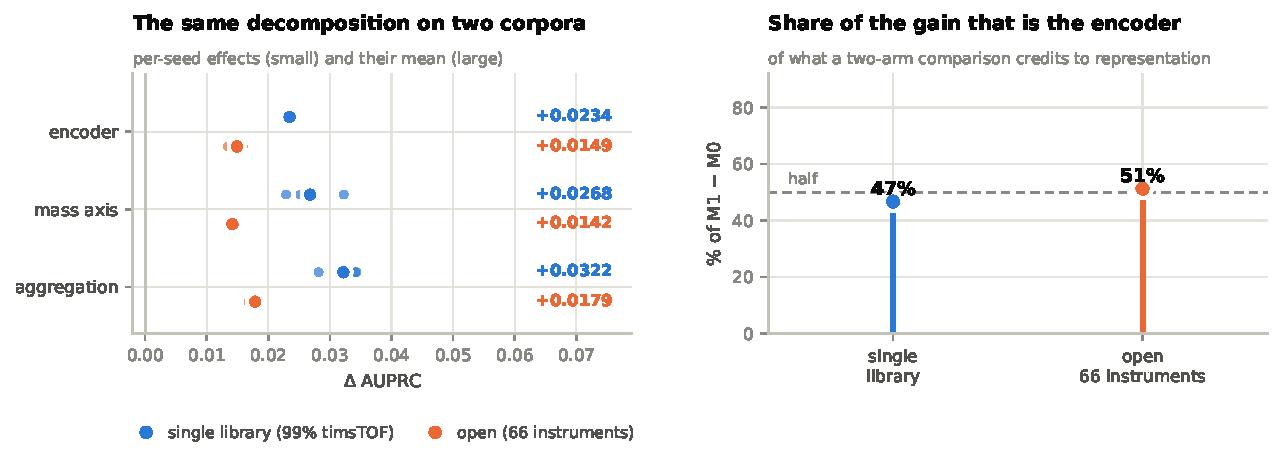
\includegraphics[width=\linewidth]{figures/fig2_two_corpora.pdf}
\caption{The decomposition on two corpora. \textbf{Left}: each effect measured on
both, with per-seed values (small) and their mean (large). \textbf{Right}: the
encoder's share of the gain a two-arm comparison would attribute to the
representation.}
\label{fig:corpora}
\end{figure}

\begin{table}[htbp]
\centering
\caption{The decomposition on two corpora. The single-library corpus is 99\% timsTOF from one in-house library; the open corpus spans 66 instrument types across GNPS, MassBank and MoNA. Absorption is measured on each corpus's own held-out spectra.}
\label{tab:table3_two_corpora}
\begin{tabular}{l r r r r}
\toprule
effect & single library & SD (single) & open corpus & SD (open) \\
\midrule
encoder & +0.0234 & 0.0002 & +0.0149 & 0.0013 \\
mass axis & +0.0268 & 0.0049 & +0.0142 & 0.0004 \\
aggregation & +0.0322 & 0.0035 & +0.0179 & 0.0009 \\
encoder share of M1 $-$ M0 & 46.7\% & -- & 51.3\% & -- \\
peaks absorbed at 0.5 Da & 34.4\% & -- & 23.6\% & -- \\
\bottomrule
\end{tabular}
\end{table}


\hd{What binning removes, and how much of it matters}
The mechanism is visible before any model is fitted. Of the $3{,}797{,}166$ peaks in
the open corpus's held-out spectra, $23.6\%$ fall into a $0.5$~Da bin already
occupied by another peak from the same spectrum and are therefore absorbed. On the
single-library corpus's held-out spectra the same figure is $34.4\%$
(Fig.~\ref{fig:absorption}). The loss falls with the grid on both, reaching $2.9\%$
and $6.5\%$ respectively at $0.01$~Da.

What a merged peak costs is compositional identity. Enumerating plausible CHNOS
compositions within $10$~ppm places $328$ candidate fragment formulas inside a
single $0.5$~Da bin at $m/z\,300$. The width of the mass window governs that count,
in the way Kind and Fiehn established for precursor formulas \cite{kind2007rules}.
A bin three orders of magnitude wider than the instrument's error therefore
discards almost all of the discrimination the measurement bought.

The two corpora move in the same direction on both quantities. The one that loses
more peaks to binning is also the one where the mass axis is worth more: $34.4\%$
and $+0.0268$ against $23.6\%$ and $+0.0142$. The correspondence is not
proportional, since absorption falls to $0.69$ of its value while the effect falls
to $0.53$. Peak absorption is therefore not a complete account of the cost, but it
does move with it.

We offer one hypothesis for the difference, which our design does not test. The
single-library corpus is almost entirely timsTOF, a high-resolution instrument on
which every reported $m/z$ carries real precision. The open corpus spans $66$
instrument types of varying resolution, and on the lower-resolution ones there is
less precision present to preserve, so the average value of preserving it falls.
Stratifying the mass-axis effect by instrument resolution would test this directly
and we regard it as the most informative experiment this work leaves undone.

\begin{figure}[htbp]
\centering
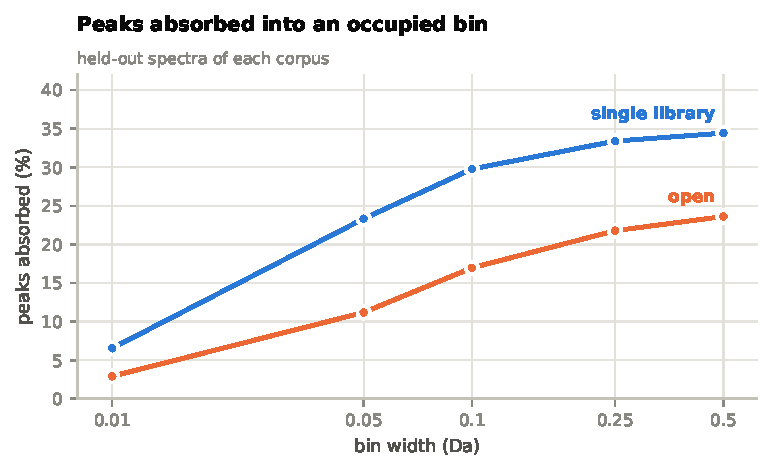
\includegraphics[width=0.62\linewidth]{figures/fig3_absorption_both.pdf}
\caption{Fraction of peaks absorbed into an already-occupied bin, against grid width,
on each corpus's own held-out spectra.}
\label{fig:absorption}
\end{figure}

\hd{How much precision is needed}
The rounding control prices one particular grid. Sweeping the grid width on the
single-library corpus, with the encoder and parameter count fixed throughout, prices
precision as a function of how much of it is retained
(Table~\ref{tab:table3_binwidth}). At $0.5$, $0.25$ and $0.1$~Da the model sits
between $0.0801$ and $0.0867$, a range of $0.0066$ --- under twice that arm's seed
standard deviation of $0.0039$, and unordered within itself; coarsening from $0.1$
to $0.5$~Da costs nothing measurable. Below that the curve moves: $0.05$~Da reaches
$0.0909$ and $0.01$~Da reaches $0.1030$, closing $65\%$ of the distance to full
precision. Even a $10$~mDa grid --- fine enough to separate the isobaric fragments
that motivate the mass-defect argument --- leaves roughly a third of the benefit
unrealised, which suggests the model uses the defect as a continuous quantity rather
than merely as a discriminator between candidate formulas.

Two cautions. Each width was run once, so the non-monotonic dip at $0.25$ and
$0.1$~Da, spanning $0.0066$, is unremarkable across five single runs and we read it
as noise rather than structure. We also tested an alternative explanation. The
sinusoidal basis has wavelengths that are integer divisors of these grid spacings,
which would render some channels constant. But only one to three of thirty-two
channels are affected at any width, and the count does not track performance
($r = -0.26$), so we discount aliasing. The sweep was run on the
single-library corpus only; whether the $0.05$~Da threshold moves with instrument
diversity is open.

\begin{table}[htbp]
\centering
\caption{Bin-width sweep, single seed. Every arm uses the M1 encoder at an identical parameter count; only the width of the mass grid changes. The final column expresses each result as a share of the distance between the 0.5 Da arm and full precision.}
\label{tab:table3_binwidth}
\begin{tabular}{l r r r}
\toprule
bin width (Da) & peaks absorbed & macro AUPRC & share of the 0.5 Da gap closed \\
\midrule
0.5 & 37.5\% & 0.0867 & 0\% \\
0.25 & 36.8\% & 0.0818 & -19\% \\
0.1 & 33.1\% & 0.0801 & -26\% \\
0.05 & 25.9\% & 0.0909 & 17\% \\
0.01 & 7.5\% & 0.1030 & 65\% \\
full precision & 0.0\% & 0.1119 & 100\% \\
\bottomrule
\end{tabular}
\end{table}

